\documentclass[xcolor=dvipsnames,aspectratio=169]{beamer}
\usepackage[utf8]{inputenc}
\usepackage[brazil]{babel}
\usepackage{graphicx,xcolor,comment,enumerate,indentfirst}
\usepackage{amsmath}
\usepackage{amsthm}
\usepackage{gensymb}
\usepackage{multicol}
\usepackage{blindtext}
\usepackage{amsfonts}
\usepackage{amssymb}
\usepackage{graphicx}
\usepackage{indentfirst}
\usepackage{wrapfig}
\usepackage{cutwin}
\usepackage{lipsum}
\usepackage{xspace,multicol}
\usepackage{ragged2e}
\usepackage{multicol}
\usepackage[backend=biber,style=abnt]{biblatex}
\usepackage{acro}
\usepackage{mathtools}
\DeclarePairedDelimiter{\ceil}{\lceil}{\rceil}
\usetheme{Madrid}
\setbeamertemplate{caption}[numbered]{}% Number floa\ust-like environments


\title{Modelagem e controle de um conversor flyback por meio de estratégias de controle preditivo.}
\author[Ricardo Machado]{\textbf{Ricardo Augusto de Araújo Machado}}
\date{\today}

\institute[UFBA]{Escola Politécnica da UFBA \\ Programa de Pós-Graduação em Engenharias Elétrica e de Computação \\[0.5em]}

\titlegraphic{
\includegraphics[height=1cm]{Figs/UFBA.jpeg} \hspace{1cm} 
\includegraphics[height=1cm]{Figs/brasao_escola_politecnica.png}}

\definecolor{english}{rgb}{0.0, 0.3, 0.5}
\usecolortheme[named = english]{structure}

\bibliography{refs.bib}


\begin{document}

\maketitle

\begin{frame}{Conversor Flyback - Introdução.}
    \justifying
    O conversor flyback é um conversor de corrente contínua extremamente popular em fontes chaveadas (SMPS) de baixa potência \cite{Picard2010}.

    A operação do conversor flyback consiste em armazenar energia na indutância de magnetização do transformador enquanto a chave conduz corrente e, em seguida, transferir essa energia armazenada para a saída enquanto a chave está aberta.
    \begin{figure}[h]
        \centering
        \caption{Diagrama de circuito do conversor flyback.}
        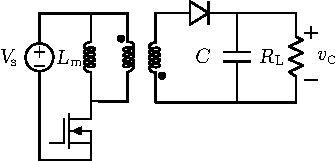
\includegraphics[width=0.5\linewidth]{Figs/flyback.pdf}
        \label{fig:diagrama_circuito}
    \end{figure}
\end{frame}


\begin{frame}{Conversor Flyback - Especificações}
    O conversor flyback é dimensionado para operar no modo de condução contínua. Ademais, a frequência de chaveamento é definida como \(50\ \mathrm{kHz}\) e a potência de saída nominal é \(6\ W\). As especificações completas são listadas na Tabela \ref{tab:specs}.
    \begin{table}[h]
        \centering
        \caption{Especificações do conversor flyback.}
        \label{tab:specs}
        \begin{tabular}{|l|l|l|}
            \hline
            Notação                          & Nome do parâmetro         & Valor         \\ \hline
            \(V_s\)                          & Tensão de entrada         & 48 V          \\ \hline
            \(V_o\)                          & Tensão de saída           & 12 V          \\ \hline
            \(f_s\)                          & Frequência de chaveamento & 50 kHz        \\ \hline
            \(P_o\)                          & Potência de saída         & 6 W           \\ \hline
            \(\frac{\Delta v_C}{V_C}\)       & Ripple de tensão          & 2\%           \\ \hline
            \(\frac{\Delta i_{Lm}}{I_{Lm}}\) & Ripple de corrente        & 30\%          \\ \hline
            \(n\)                            & Razão entre espiras       & 0,25          \\ \hline
            \(R_L\)                          & Resistor de carga         & 24 \(\Omega\) \\ \hline
        \end{tabular}
    \end{table}

\end{frame}

\begin{frame}{Conversor Flyback - Modelagem}
    A modelagem do conversor flyback, descrita em \cite{Erickson2020} e \cite{Hart2012}, consiste na determinação das equações dinâmicas da tensão no indutor e da corrente no capacitor durante os dois estados de operação do conversor, chave fechada (ON) e chave aberta (OFF), as quais são descritas em  \eqref{eq:estado_on} e \eqref{eq:estado_off}, respectivamente.

    \begin{equation}
        \begin{cases}
            \dfrac{di_{Lm}}{dt} = \dfrac{V_s}{L_m} \\ \\
            \dfrac{dv_c}{dt} = -\dfrac{v_c}{RC}
        \end{cases}
        \label{eq:estado_on}
    \end{equation}


    \begin{equation}
        \begin{cases}
            \dfrac{d i_{Lm}}{dt} = - \dfrac{v_c}{n \cdot L_m} \\ \\
            \dfrac{dv_c}{dt} = \dfrac{i_{Lm}}{n \cdot C} - \dfrac{v_c}{RC}
        \end{cases}
        \label{eq:estado_off}
    \end{equation}

\end{frame}

\begin{frame}{Conversor Flyback - Modelo Médio}
    Neste trabalho, o efeito da comutação no conversor é desprezado, pois tanto o projeto do sistema de controle, quanto as simulações são realizadas com base no modelo dinâmico médio do conversor, descrito em \eqref{eq:modelo_medio}. A saída do sistema é definida como a tensão no capacitor.

    \begin{equation}
        \begin{cases}
            \dfrac{d i_{Lm}}{dt} = - \dfrac{(1-d)}{n \cdot L_m} v_c + \dfrac{d}{L_m} V_s \\ \\
            \dfrac{dv_c}{dt} = \dfrac{(1-d)}{n \cdot C} i_{Lm} - \dfrac{1}{RC} v_c       \\ \\
            y = v_c
        \end{cases}
        \label{eq:modelo_medio}
    \end{equation}
\end{frame}

\begin{frame}{Dimensionamento do conversor.}
    \justifying
    As expressões para a tensão média no capacitor e para a corrente média no indutor, dadas por \eqref{eq:tensao_media} e \eqref{eq:corrente_media}, são obtidas por meio do balanço Volt-Segundo no indutor e do balanço de carga no capacitor, respectivamente.
    Para as tensões nominais definidas no projeto do conversor, a razão cíclica de equilibrio obtida é \(D = 0,5\).

    \begin{equation}
        V_\mathrm{C} = \frac{n V_s D}{(1 - D)} \Rightarrow V_\mathrm{C} = 12 \ \mathrm{V}
        \label{eq:tensao_media}
    \end{equation}

    \begin{equation}
        I_\mathrm{Lm} = \frac{n V_c}{R \cdot (1-D)} \Rightarrow  I_\mathrm{Lm} = 0,25 \ \mathrm{A}
        \label{eq:corrente_media}
    \end{equation}


\end{frame}

\begin{frame}{Dimensionamento do conversor.}
    \justifying
    A capacitância e a indutância do conversor são determinadas com base nas especificações do ripple de tensão e ripple de corrente \cite{Erickson2020}, respectivamente, conforme \eqref{eq:capacitor_flyback} e \eqref{eq:indutor_flyback}.

    \begin{equation}
        C = \frac{D}{Rs f_s \frac{|\Delta v_c|}{V_c}} \Rightarrow C = 20.833\ \mathrm{\mu F}
        \label{eq:capacitor_flyback}
    \end{equation}

    \begin{equation}
        L  =\frac{R(1-D)^2}{n^2 f_s \frac{|\Delta i_{Lm}|}{I_{Lm}}} \Rightarrow L = 6.4\ \mathrm{mH}
        \label{eq:indutor_flyback}
    \end{equation}

\end{frame}

\begin{frame}{Ponto de equilibrio do conversor.}

    O vetor de estados é representado por \(\mathbf{x}\), o vetor de estados no equilibrio por \(\mathbf{X}\) e o vetor de desvio dos estados em relação ao equilibrio por \(\mathbf{\hat{x}}\) (Eq. \eqref{eq:vetor_estados}).
    O ponto de equilibrio é descrito em \eqref{eq:ponto_equilibrio}.

    \begin{equation}
        \mathbf{x} = \begin{bmatrix}
            i_{Lm} \\
            v_C
        \end{bmatrix}
        \qquad   \mathbf{X} = \begin{bmatrix}
            I_{Lm} \\
            V_C
        \end{bmatrix}
        \qquad \mathbf{\hat{x}} = \begin{bmatrix}
            \hat{i}_{Lm} \\
            \hat{v}_C
        \end{bmatrix} =  \begin{bmatrix}
            i_{Lm} - I_{Lm} \\
            v_C - V_C
        \end{bmatrix}
        \label{eq:vetor_estados}
    \end{equation}

    \begin{equation}
        \mathbf{U} = 0,5 \qquad \mathbf{X} =
        \begin{bmatrix}
            0,25\ \mathrm{A} \\
            12 \ \mathrm{V}
        \end{bmatrix}
        \label{eq:ponto_equilibrio}
    \end{equation}

\end{frame}

\begin{frame}{Modelo linearizado.}
    \justifying
    O modelo linearizado do conversor em espaço de estados (Eq. \eqref{eq:modelo_ss}) é obtido com a determinação do Jacobiano do sistema em relação aos estados e em relação à entrada. As matrizes \(A\), \(B\) e \(C\) do modelo são descritas em \eqref{eq:matriz_a}, \eqref{eq:matriz_b} e \eqref{eq:matriz_c}.

    \begin{equation}
        A =
        \begin{bmatrix}
            0                     & - \frac{1-D}{n\cdot L_m} \\ \\
            \frac{1-D}{n \cdot C} & -\frac{1}{R C}
        \end{bmatrix}
        \label{eq:matriz_a}
    \end{equation}

    \begin{equation}
        B =
        \begin{bmatrix}
            \frac{V_c}{n \cdot L_m} + \frac{V_s}{L_m} \\ \\
            \frac{- I_{Lm}}{n \cdot C}
        \end{bmatrix}
        \label{eq:matriz_b}
    \end{equation}

    \begin{equation}
        C = \begin{bmatrix}
            0 & 1
        \end{bmatrix}
        \label{eq:matriz_c}
    \end{equation}

    \begin{equation}
        \begin{cases}
            \frac{d \mathbf{\hat{x}}}{d t} = A\ \mathbf{\hat{x}} + B\ \hat{u} \\
            \hat{y} = C\ \mathbf{\hat{x}}
        \end{cases}
        \label{eq:modelo_ss}
    \end{equation}

\end{frame}

\begin{frame}{Modelo linearizado - Valores numéricos.}
    \justifying
    Os valores numéricos para as matrizes do modelo em espaço de estados são descritas em \eqref{eq:matriz_a_num}, \eqref{eq:matriz_b_num} e \eqref{eq:matriz_c_num}.

    \begin{equation}
        A =
        \begin{bmatrix}
            0     & -312,50 \\
            96000 & -2000
        \end{bmatrix}
        \label{eq:matriz_a_num}
    \end{equation}

    \begin{equation}
        B =
        \begin{bmatrix}
            15000 \\
            -48000
        \end{bmatrix}
        \label{eq:matriz_b_num}
    \end{equation}

    \begin{equation}
        C = \begin{bmatrix}
            0 & 1
        \end{bmatrix}
        \label{eq:matriz_c_num}
    \end{equation}
\end{frame}

\begin{frame}{Validação do modelo linearizado.}

    A validação do modelo linearizado é realizado através da comparação entre a simulação de \textit{AC Sweep} do conversor para uma perturbação senoidal no \textit{duty cycle} (Fig. \ref{fig:diagrama_sim}) e a resposta em frequência do modelo linearizado. A perturbação senoidal tem amplitude de 0,01 e frequência variável entre 100 Hz e 10 kHz.

    \begin{figure}[htb]
        \centering
        \caption{Diagrama da simulação \textit{AC Sweep} realizada no PSIM.}
        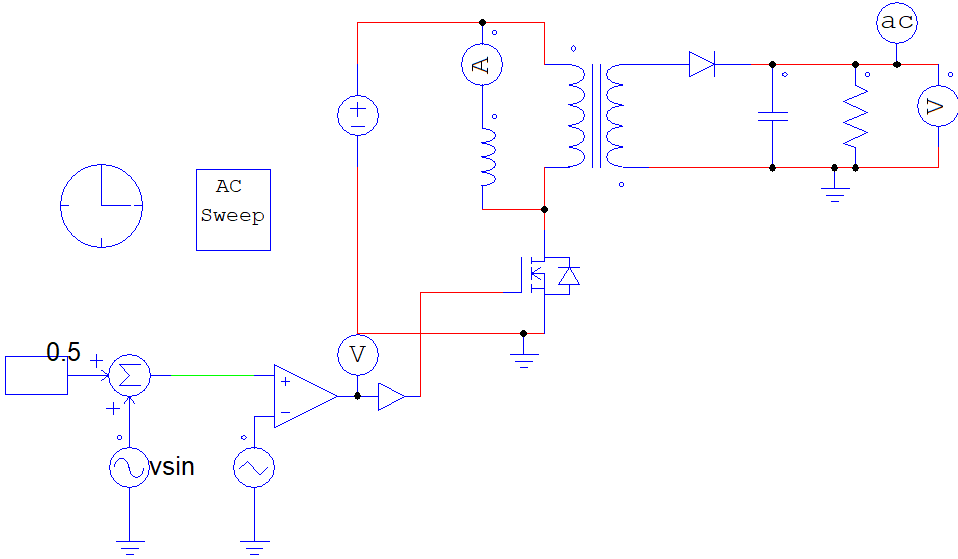
\includegraphics[width=0.45\textwidth]{Figs/Diagrama Simulação.png}
        \label{fig:diagrama_sim}
    \end{figure}

\end{frame}


\begin{frame}{Validação do modelo linearizado.}

    A Figura \ref{fig:comp_resp_freq} ilustra a comparação entre a simulação de \textit{AC Sweep} do conversor e a reposta em frequência do modelo linearizado.

    \begin{figure}[htb]
        \centering
        \caption{Comparação entre simulação AC e resposta em frequência do modelo.}
        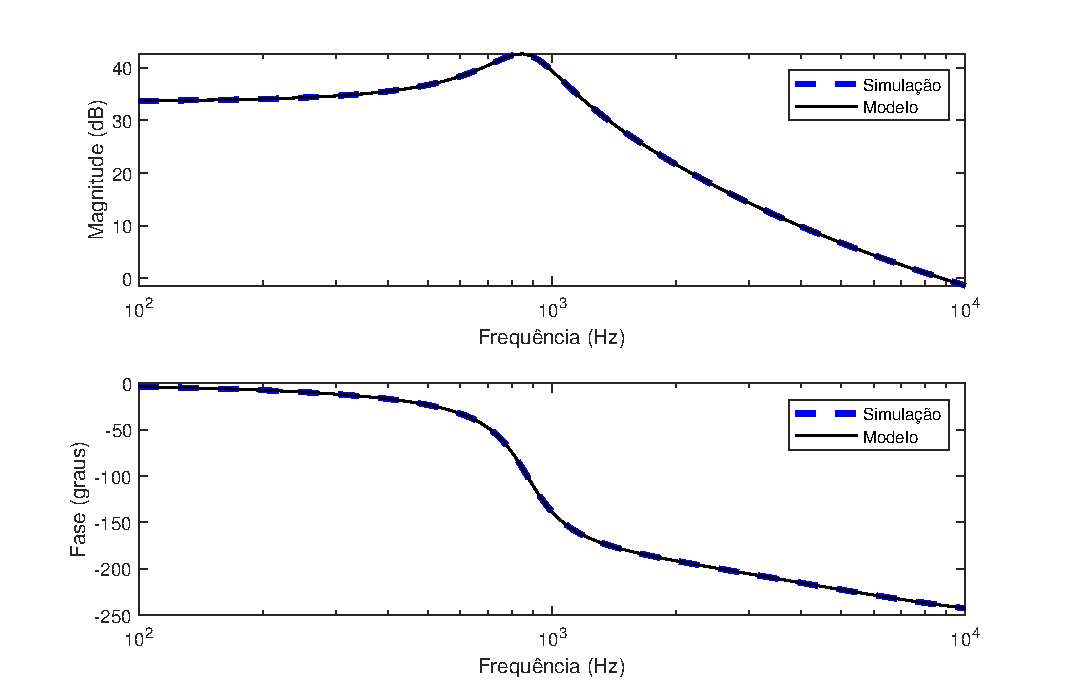
\includegraphics[width=0.55\textwidth]{Figs/Valid Modelo.pdf}
        \label{fig:comp_resp_freq}
    \end{figure}

\end{frame}

\begin{frame}[allowframebreaks, noframenumbering]
    \frametitle{Referências}
    \printbibliography
\end{frame}


\end{document}
